\documentclass[12pt, twoside]{article}
\usepackage[letterpaper, margin=1in, headsep=0.5in]{geometry}
\usepackage[english]{babel}
\usepackage[utf8]{inputenc}
\usepackage{amsmath}
\usepackage{amsfonts}
\usepackage{amssymb}
\usepackage{tikz}
%\usetikzlibrary{quotes, angles}

\usepackage{graphicx}
\usepackage{enumitem}
\usepackage{multicol}

\usepackage{fancyhdr}
\pagestyle{fancy}
\fancyhf{}
\renewcommand{\headrulewidth}{0pt} % disable the underline of the header

\fancyhead[RE]{\thepage}
\fancyhead[RO]{\thepage \\ Name: \hspace{3cm}}
\fancyhead[L]{BECA / Dr. Huson / 10th Grade Geometry\\* 2 April 2019}

\begin{document}
\subsubsection*{Test: Mock Regents Geometry Exam}

Use the last four digits of your student number as your Gradecam ID. Write the number and bubble in your ID (1 point).\\[0.5cm]

Answer the \textbf{Free Response first }, then the multiple choice questions. Turn in this answer sheet and the Free Response section. Keep the multiple choice questions for test corrections. \\[0.5cm]

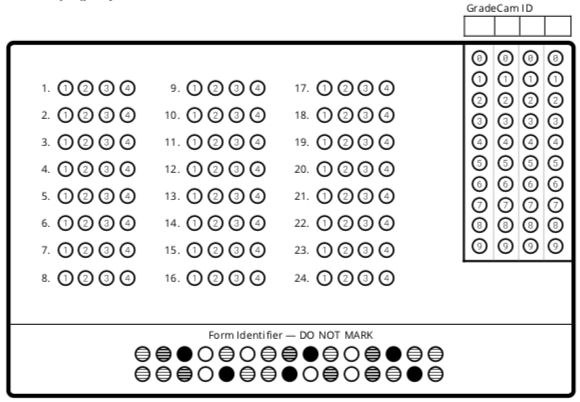
\includegraphics[width=0.9\textwidth]{gradecam-24.png}


\end{document}
